\documentclass[10pt,a4paper]{tufte-handout}

% ams
\usepackage{amssymb,amsmath}

\usepackage{ifxetex,ifluatex}
\usepackage{fixltx2e} % provides \textsubscript
\ifnum 0\ifxetex 1\fi\ifluatex 1\fi=0 % if pdftex
  \usepackage[T1]{fontenc}
  \usepackage[utf8]{inputenc}
\else % if luatex or xelatex
  \makeatletter
  \@ifpackageloaded{fontspec}{}{\usepackage{fontspec}}
  \makeatother
  \defaultfontfeatures{Ligatures=TeX,Scale=MatchLowercase}
  \makeatletter
  \@ifpackageloaded{soul}{
     \renewcommand\allcapsspacing[1]{{\addfontfeature{LetterSpace=15}#1}}
     \renewcommand\smallcapsspacing[1]{{\addfontfeature{LetterSpace=10}#1}}
   }{}
  \makeatother
\fi

% graphix
\usepackage{graphicx}
\setkeys{Gin}{width=\linewidth,totalheight=\textheight,keepaspectratio}

% booktabs
\usepackage{booktabs}

% url
\usepackage{url}

% hyperref
\usepackage{hyperref}

% units.
\usepackage{units}


\setcounter{secnumdepth}{2}

% citations
\usepackage{natbib}
\bibliographystyle{biblio/ecology}

% pandoc syntax highlighting
\usepackage{color}
\usepackage{fancyvrb}
\newcommand{\VerbBar}{|}
\newcommand{\VERB}{\Verb[commandchars=\\\{\}]}
\DefineVerbatimEnvironment{Highlighting}{Verbatim}{commandchars=\\\{\}}
% Add ',fontsize=\small' for more characters per line
\usepackage{framed}
\definecolor{shadecolor}{RGB}{248,248,248}
\newenvironment{Shaded}{\begin{snugshade}}{\end{snugshade}}
\newcommand{\AlertTok}[1]{\textcolor[rgb]{0.94,0.16,0.16}{#1}}
\newcommand{\AnnotationTok}[1]{\textcolor[rgb]{0.56,0.35,0.01}{\textbf{\textit{#1}}}}
\newcommand{\AttributeTok}[1]{\textcolor[rgb]{0.77,0.63,0.00}{#1}}
\newcommand{\BaseNTok}[1]{\textcolor[rgb]{0.00,0.00,0.81}{#1}}
\newcommand{\BuiltInTok}[1]{#1}
\newcommand{\CharTok}[1]{\textcolor[rgb]{0.31,0.60,0.02}{#1}}
\newcommand{\CommentTok}[1]{\textcolor[rgb]{0.56,0.35,0.01}{\textit{#1}}}
\newcommand{\CommentVarTok}[1]{\textcolor[rgb]{0.56,0.35,0.01}{\textbf{\textit{#1}}}}
\newcommand{\ConstantTok}[1]{\textcolor[rgb]{0.00,0.00,0.00}{#1}}
\newcommand{\ControlFlowTok}[1]{\textcolor[rgb]{0.13,0.29,0.53}{\textbf{#1}}}
\newcommand{\DataTypeTok}[1]{\textcolor[rgb]{0.13,0.29,0.53}{#1}}
\newcommand{\DecValTok}[1]{\textcolor[rgb]{0.00,0.00,0.81}{#1}}
\newcommand{\DocumentationTok}[1]{\textcolor[rgb]{0.56,0.35,0.01}{\textbf{\textit{#1}}}}
\newcommand{\ErrorTok}[1]{\textcolor[rgb]{0.64,0.00,0.00}{\textbf{#1}}}
\newcommand{\ExtensionTok}[1]{#1}
\newcommand{\FloatTok}[1]{\textcolor[rgb]{0.00,0.00,0.81}{#1}}
\newcommand{\FunctionTok}[1]{\textcolor[rgb]{0.00,0.00,0.00}{#1}}
\newcommand{\ImportTok}[1]{#1}
\newcommand{\InformationTok}[1]{\textcolor[rgb]{0.56,0.35,0.01}{\textbf{\textit{#1}}}}
\newcommand{\KeywordTok}[1]{\textcolor[rgb]{0.13,0.29,0.53}{\textbf{#1}}}
\newcommand{\NormalTok}[1]{#1}
\newcommand{\OperatorTok}[1]{\textcolor[rgb]{0.81,0.36,0.00}{\textbf{#1}}}
\newcommand{\OtherTok}[1]{\textcolor[rgb]{0.56,0.35,0.01}{#1}}
\newcommand{\PreprocessorTok}[1]{\textcolor[rgb]{0.56,0.35,0.01}{\textit{#1}}}
\newcommand{\RegionMarkerTok}[1]{#1}
\newcommand{\SpecialCharTok}[1]{\textcolor[rgb]{0.00,0.00,0.00}{#1}}
\newcommand{\SpecialStringTok}[1]{\textcolor[rgb]{0.31,0.60,0.02}{#1}}
\newcommand{\StringTok}[1]{\textcolor[rgb]{0.31,0.60,0.02}{#1}}
\newcommand{\VariableTok}[1]{\textcolor[rgb]{0.00,0.00,0.00}{#1}}
\newcommand{\VerbatimStringTok}[1]{\textcolor[rgb]{0.31,0.60,0.02}{#1}}
\newcommand{\WarningTok}[1]{\textcolor[rgb]{0.56,0.35,0.01}{\textbf{\textit{#1}}}}

% longtable
\usepackage{longtable,booktabs}

% multiplecol
\usepackage{multicol}

% strikeout
\usepackage[normalem]{ulem}

% morefloats
\usepackage{morefloats}


% tightlist macro required by pandoc >= 1.14
\providecommand{\tightlist}{%
  \setlength{\itemsep}{0pt}\setlength{\parskip}{0pt}}

% title / author / date
\title{Distance sampling online workshop}
\author{Analysis in R: Analysis of multi-species surveys}
\date{CREEM, Univ of St Andrews -- October 2018}

%% -- tint overrides
%% fonts, using roboto (condensed) as default
\usepackage[sfdefault,condensed]{roboto}
%% also nice: \usepackage[default]{lato}

%% colored links, setting 'borrowed' from RJournal.sty with 'Thanks, Achim!'
\RequirePackage{color}
\definecolor{link}{rgb}{0.1,0.1,0.8} %% blue with some grey
\hypersetup{
  colorlinks,%
  citecolor=link,%
  filecolor=link,%
  linkcolor=link,%
  urlcolor=link
}

%% macros
\makeatletter

%% -- tint does not use italics or allcaps in title
\renewcommand{\maketitle}{%     
  \newpage
  \global\@topnum\z@% prevent floats from being placed at the top of the page
  \begingroup
    \setlength{\parindent}{0pt}%
    \setlength{\parskip}{4pt}%
    \let\@@title\@empty
    \let\@@author\@empty
    \let\@@date\@empty
    \ifthenelse{\boolean{@tufte@sfsidenotes}}{%
      %\gdef\@@title{\sffamily\LARGE\allcaps{\@title}\par}%
      %\gdef\@@author{\sffamily\Large\allcaps{\@author}\par}%
      %\gdef\@@date{\sffamily\Large\allcaps{\@date}\par}%
      \gdef\@@title{\begingroup\fontseries{b}\selectfont\LARGE{\@title}\par}%
      \gdef\@@author{\begingroup\fontseries{l}\selectfont\Large{\@author}\par}%
      \gdef\@@date{\begingroup\fontseries{l}\selectfont\Large{\@date}\par}%
    }{%
      %\gdef\@@title{\LARGE\itshape\@title\par}%
      %\gdef\@@author{\Large\itshape\@author\par}%
      %\gdef\@@date{\Large\itshape\@date\par}%
      \gdef\@@title{\begingroup\fontseries{b}\selectfont\LARGE\@title\par\endgroup}%
      \gdef\@@author{\begingroup\fontseries{l}\selectfont\Large\@author\par\endgroup}%
      \gdef\@@date{\begingroup\fontseries{l}\selectfont\Large\@date\par\endgroup}%
    }%
    \@@title
    \@@author
    \@@date
  \endgroup
  \thispagestyle{plain}% suppress the running head
  \tuftebreak% add some space before the text begins
  \@afterindentfalse\@afterheading% suppress indentation of the next paragraph
}

%% -- tint does not use italics or allcaps in section/subsection/paragraph
\titleformat{\section}%
  [hang]% shape
  %{\normalfont\Large\itshape}% format applied to label+text
  {\fontseries{b}\selectfont\Large}% format applied to label+text
  {\thesection}% label
  {1em}% horizontal separation between label and title body
  {}% before the title body
  []% after the title body

\titleformat{\subsection}%
  [hang]% shape
  %{\normalfont\large\itshape}% format applied to label+text
  {\fontseries{m}\selectfont\large}% format applied to label+text
  {\thesubsection}% label
  {1em}% horizontal separation between label and title body
  {}% before the title body
  []% after the title body

\titleformat{\paragraph}%
  [runin]% shape
  %{\normalfont\itshape}% format applied to label+text
  {\fontseries{l}\selectfont}% format applied to label+text
  {\theparagraph}% label
  {1em}% horizontal separation between label and title body
  {}% before the title body
  []% after the title body

%% -- tint does not use italics here either
% Formatting for main TOC (printed in front matter)
% {section} [left] {above} {before w/label} {before w/o label} {filler + page} [after]
\ifthenelse{\boolean{@tufte@toc}}{%
  \titlecontents{part}% FIXME
    [0em] % distance from left margin
    %{\vspace{1.5\baselineskip}\begin{fullwidth}\LARGE\rmfamily\itshape} % above (global formatting of entry)
    {\vspace{1.5\baselineskip}\begin{fullwidth}\fontseries{m}\selectfont\LARGE} % above (global formatting of entry)
    {\contentslabel{2em}} % before w/label (label = ``II'')
    {} % before w/o label
    {\rmfamily\upshape\qquad\thecontentspage} % filler + page (leaders and page num)
    [\end{fullwidth}] % after
  \titlecontents{chapter}%
    [0em] % distance from left margin
    %{\vspace{1.5\baselineskip}\begin{fullwidth}\LARGE\rmfamily\itshape} % above (global formatting of entry)
    {\vspace{1.5\baselineskip}\begin{fullwidth}\fontseries{m}\selectfont\LARGE} % above (global formatting of entry)
    {\hspace*{0em}\contentslabel{2em}} % before w/label (label = ``2'')
    {\hspace*{0em}} % before w/o label
    %{\rmfamily\upshape\qquad\thecontentspage} % filler + page (leaders and page num)
    {\upshape\qquad\thecontentspage} % filler + page (leaders and page num)
    [\end{fullwidth}] % after
  \titlecontents{section}% FIXME
    [0em] % distance from left margin
    %{\vspace{0\baselineskip}\begin{fullwidth}\Large\rmfamily\itshape} % above (global formatting of entry)
    {\vspace{0\baselineskip}\begin{fullwidth}\fontseries{m}\selectfont\Large} % above (global formatting of entry)
    {\hspace*{2em}\contentslabel{2em}} % before w/label (label = ``2.6'')
    {\hspace*{2em}} % before w/o label
    %{\rmfamily\upshape\qquad\thecontentspage} % filler + page (leaders and page num)
    {\upshape\qquad\thecontentspage} % filler + page (leaders and page num)
    [\end{fullwidth}] % after
  \titlecontents{subsection}% FIXME
    [0em] % distance from left margin
    %{\vspace{0\baselineskip}\begin{fullwidth}\large\rmfamily\itshape} % above (global formatting of entry)
    {\vspace{0\baselineskip}\begin{fullwidth}\fontseries{m}\selectfont\large} % above (global formatting of entry)
    {\hspace*{4em}\contentslabel{4em}} % before w/label (label = ``2.6.1'')
    {\hspace*{4em}} % before w/o label
    %{\rmfamily\upshape\qquad\thecontentspage} % filler + page (leaders and page num)
    {\upshape\qquad\thecontentspage} % filler + page (leaders and page num)
    [\end{fullwidth}] % after
  \titlecontents{paragraph}% FIXME
    [0em] % distance from left margin
    %{\vspace{0\baselineskip}\begin{fullwidth}\normalsize\rmfamily\itshape} % above (global formatting of entry)
    {\vspace{0\baselineskip}\begin{fullwidth}\fontseries{m}\selectfont\normalsize\rmfamily} % above (global formatting of entry)
    {\hspace*{6em}\contentslabel{2em}} % before w/label (label = ``2.6.0.0.1'')
    {\hspace*{6em}} % before w/o label
    %{\rmfamily\upshape\qquad\thecontentspage} % filler + page (leaders and page num)
    {\upshape\qquad\thecontentspage} % filler + page (leaders and page num)
    [\end{fullwidth}] % after
}{}

  
\makeatother



\begin{document}

\maketitle




\hypertarget{more-complex-analyses}{%
\section{More complex analyses}\label{more-complex-analyses}}

\begin{marginfigure}
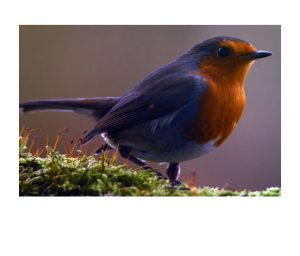
\includegraphics[]{images/robin-300x256.jpg} European robin
\emph{(Erithacus rubecula)}; one of the species in the Montrave study of
\citet{Buckland_2006}.
\end{marginfigure}

This practical is based on the Montrave songbird case study in
\citet{buckland_distance_2015}, with computer code under
\href{https://synergy.st-andrews.ac.uk/ds-manda/\#montrave-songbird-case-study}{Montrave
songbird case study}. Both point and line transect surveys were
conducted and here we use the data from the \textbf{line transect} data,
although the issues (and solutions) will be similar.

These data are provided in a `flat file' format (i.e.~it contains all
the necessary columns to estimate a detection function, density and
abundance). While both formats are equally valid, the `flat file'
approach has a particular idiosyncrasy which we exploit here to
introduce more functions and data manipulation.

Several species of birds were identified but not all species were
detected on all transects. If a simple data selection is performed to
select records for a particular species, then not all of the transects
will be included in the resulting data (because that species may not
have been seen). This doesn't matter if we are only interested in
fitting detection functions, but will matter if we wish to estimate
density and abundance because the effort will be too low since some of
the transects are missing. To correct for this, some data frame
manipulation is required. There is generally more than one way to do
something in R \citep{r_language} - for an alternative way see the
computer code `Montrave song bird case study' associated with
\citet{buckland_distance_2015}.

\hypertarget{objectives-of-the-practical}{%
\subsection{Objectives of the
practical}\label{objectives-of-the-practical}}

\begin{enumerate}
\def\labelenumi{\arabic{enumi}.}
\tightlist
\item
  Data frame selection and manipulation
\item
  Extracting estimates from \texttt{dht} object
\item
  Customising detection function plots
\end{enumerate}

\hypertarget{importing-the-data}{%
\subsection{Importing the data}\label{importing-the-data}}

The data is in a `flat file' format and contains the following columns:

\begin{itemize}
\tightlist
\item
  Region.Label - name of study
\item
  Area - size of study region (km\(^2\))
\item
  repeats - number of visits to transect
\item
  Sample.Label - line transect identifier
\item
  Effort - length of transect (km)
\item
  distance - perpendicular distance (m)
\item
  species - species of bird (c=chaffinch, g=great tit, r=robin and w
  =wren)
\item
  visit - on which visit bird was detected.
\end{itemize}

Use the following command to import the data and then use the
\texttt{head} command to ensure it has been imported correctly.

\begin{Shaded}
\begin{Highlighting}[]
\NormalTok{birds <-}\StringTok{ }\KeywordTok{read.csv}\NormalTok{(}\StringTok{"datasets/montrave-line.csv"}\NormalTok{, }
    \DataTypeTok{header =} \OtherTok{TRUE}\NormalTok{)}
\end{Highlighting}
\end{Shaded}

\begin{Shaded}
\begin{Highlighting}[]
\KeywordTok{head}\NormalTok{(birds, }\DataTypeTok{n =} \DecValTok{2}\NormalTok{)}
\end{Highlighting}
\end{Shaded}

\begin{verbatim}
##   Region.Label Area repeats Sample.Label
## 1     Montrave 33.2       2            1
## 2     Montrave 33.2       2            1
##   Effort distance species visit
## 1  0.208       75       c     1
## 2  0.208       40       c     1
\end{verbatim}

\begin{marginfigure}
\textbf{Question:} Explore the data. How many transects are there?
\end{marginfigure}

\begin{Shaded}
\begin{Highlighting}[]
\KeywordTok{length}\NormalTok{(}\KeywordTok{unique}\NormalTok{(birds}\OperatorTok{$}\NormalTok{Sample.Label))}
\end{Highlighting}
\end{Shaded}

\begin{verbatim}
## [1] 19
\end{verbatim}

For now, save the transect labels to a new object as we will use them
later on:

\begin{Shaded}
\begin{Highlighting}[]
\NormalTok{tran.lab <-}\StringTok{ }\KeywordTok{unique}\NormalTok{(birds}\OperatorTok{$}\NormalTok{Sample.Label)}
\end{Highlighting}
\end{Shaded}

The \texttt{table} command is a quick way to determine how many
detections there are of each species:

\begin{Shaded}
\begin{Highlighting}[]
\KeywordTok{table}\NormalTok{(birds}\OperatorTok{$}\NormalTok{species)}
\end{Highlighting}
\end{Shaded}

\begin{verbatim}
## 
##   c   g   r   w 
##  73  32  82 156
\end{verbatim}

As a hint of things to come, create a two-way table showing the number
of detections by transect and by species. If there are zeroes in this
table, it will create a challenge.

\begin{Shaded}
\begin{Highlighting}[]
\KeywordTok{with}\NormalTok{(birds, }\KeywordTok{table}\NormalTok{(species, Sample.Label))}
\end{Highlighting}
\end{Shaded}

\begin{longtable}[]{@{}lrrrrrrrrrrrrrrrrrrr@{}}
\toprule
& 1 & 2 & 3 & 4 & 5 & 6 & 7 & 8 & 9 & 10 & 11 & 12 & 13 & 14 & 15 & 16 &
17 & 18 & 19\tabularnewline
\midrule
\endhead
c & 4 & 7 & 7 & 5 & 9 & 7 & 5 & 1 & 1 & 3 & 1 & 0 & 2 & 2 & 4 & 3 & 4 &
7 & 1\tabularnewline
g & 0 & 2 & 3 & 5 & 5 & 1 & 3 & 2 & 1 & 1 & 0 & 0 & 2 & 0 & 2 & 0 & 3 &
1 & 1\tabularnewline
r & 3 & 8 & 11 & 5 & 8 & 7 & 5 & 7 & 3 & 1 & 0 & 2 & 5 & 6 & 4 & 0 & 4 &
3 & 0\tabularnewline
w & 10 & 11 & 12 & 11 & 14 & 12 & 13 & 11 & 6 & 3 & 1 & 4 & 9 & 12 & 9 &
2 & 7 & 6 & 3\tabularnewline
\bottomrule
\end{longtable}

Each of the line transects was visited twice which is not taken into
account at present. However, it is straightforward to do so:

\begin{Shaded}
\begin{Highlighting}[]
\NormalTok{birds}\OperatorTok{$}\NormalTok{Effort <-}\StringTok{ }\NormalTok{birds}\OperatorTok{$}\NormalTok{Effort }\OperatorTok{*}\StringTok{ }\NormalTok{birds}\OperatorTok{$}\NormalTok{repeats}
\end{Highlighting}
\end{Shaded}

\hypertarget{manipulating-the-robin-data}{%
\subsection{Manipulating the robin
data}\label{manipulating-the-robin-data}}

For the purposes of this practical, we are interested in estimating the
density of robins and so we select only these records:

\begin{Shaded}
\begin{Highlighting}[]
\NormalTok{robins <-}\StringTok{ }\NormalTok{birds[birds}\OperatorTok{$}\NormalTok{species }\OperatorTok{==}\StringTok{ "r"}\NormalTok{, ]}
\end{Highlighting}
\end{Shaded}

\begin{marginfigure}
\textbf{Question:} On how many transects were robins detected?
\end{marginfigure}

\begin{Shaded}
\begin{Highlighting}[]
\KeywordTok{length}\NormalTok{(}\KeywordTok{unique}\NormalTok{(robins}\OperatorTok{$}\NormalTok{Sample.Label))}
\end{Highlighting}
\end{Shaded}

\begin{verbatim}
## [1] 16
\end{verbatim}

If we were to use the \texttt{robins} data as it is at present to
estimate density, then density would be \textbf{incorrect} because the
search effort associated with three transects is missing. Adding these
missing transects to the \texttt{robins} data, requires several steps:

\begin{enumerate}
\def\labelenumi{\arabic{enumi}.}
\tightlist
\item
  identify the missing transects,
\item
  select the information for the missing transects,
\item
  get the missing information in the correct format,
\item
  add the missing information to the \texttt{robins} data.
\end{enumerate}

The following commands identifies the missing commands. After each
command, type the name of the object which has been created to see what
each command has done.

\begin{Shaded}
\begin{Highlighting}[]
\NormalTok{robin.lab <-}\StringTok{ }\KeywordTok{unique}\NormalTok{(robins}\OperatorTok{$}\NormalTok{Sample.Label)}
\NormalTok{miss.lab <-}\StringTok{ }\NormalTok{tran.lab[}\OperatorTok{!}\KeywordTok{is.element}\NormalTok{(}\DataTypeTok{el =}\NormalTok{ tran.lab, }
    \DataTypeTok{set =}\NormalTok{ robin.lab)]}
\end{Highlighting}
\end{Shaded}

To understand what this latter command has done, it can be broken down
into several elements:

\begin{itemize}
\tightlist
\item
  elements of \texttt{tran.lab} are selected using \texttt{{[}{]}}
\item
  the \texttt{is.element} function (without the \texttt{!} symbol)
  selects the elements in \texttt{tran.lab}, which are also in the
  \texttt{set} argument (i.e. \texttt{robin.lab})
\item
  the \texttt{!} is used to select the elements in \texttt{tran.lab}
  that are NOT in \texttt{robin.lab}.
\end{itemize}

\begin{verbatim}
## Robins were detected on the following transects:
\end{verbatim}

\begin{verbatim}
##  [1]  1  2  3  4  5  6  7  8  9 10 12 13 14
## [14] 15 17 18
\end{verbatim}

\begin{verbatim}
## 
##  Therefore missing transects are:
\end{verbatim}

\begin{verbatim}
## [1] 11 16 19
\end{verbatim}

Now we know which transects are missing, we can select these records
from the \texttt{birds} data frame:

\begin{Shaded}
\begin{Highlighting}[]
\NormalTok{miss.data <-}\StringTok{ }\NormalTok{birds[}\KeywordTok{is.element}\NormalTok{(birds}\OperatorTok{$}\NormalTok{Sample.Label, }
\NormalTok{    miss.lab), ]}
\end{Highlighting}
\end{Shaded}

However, the information about the transects are repeated in this new
data frame because we have just selected all records for these
transects. A quick check of the number of rows will confirm this:

\begin{Shaded}
\begin{Highlighting}[]
\KeywordTok{length}\NormalTok{(miss.data}\OperatorTok{$}\NormalTok{Sample.Label)}
\end{Highlighting}
\end{Shaded}

To get rid of rows where \texttt{Sample.Label} is duplicated use the
command:

\begin{Shaded}
\begin{Highlighting}[]
\NormalTok{miss.data <-}\StringTok{ }\NormalTok{miss.data[}\OperatorTok{!}\KeywordTok{duplicated}\NormalTok{(miss.data}\OperatorTok{$}\NormalTok{Sample.Label), }
\NormalTok{    ]}
\end{Highlighting}
\end{Shaded}

This command has selected the records from \texttt{miss.data} for which
the transect label is not duplicated.

We only want to keep the information about search effort and so data in
the \texttt{distance}, \texttt{species} and \texttt{visit} columns are
set to missing:

\begin{Shaded}
\begin{Highlighting}[]
\NormalTok{miss.data}\OperatorTok{$}\NormalTok{distance <-}\StringTok{ }\KeywordTok{rep}\NormalTok{(}\OtherTok{NA}\NormalTok{, }\DecValTok{3}\NormalTok{)}
\NormalTok{miss.data}\OperatorTok{$}\NormalTok{species <-}\StringTok{ }\KeywordTok{rep}\NormalTok{(}\StringTok{"NA"}\NormalTok{, }\DecValTok{3}\NormalTok{)}
\NormalTok{miss.data}\OperatorTok{$}\NormalTok{visit <-}\StringTok{ }\KeywordTok{rep}\NormalTok{(}\OtherTok{NA}\NormalTok{, }\DecValTok{3}\NormalTok{)}
\end{Highlighting}
\end{Shaded}

Examine \texttt{miss.data}.

\begin{Shaded}
\begin{Highlighting}[]
\NormalTok{miss.data}
\end{Highlighting}
\end{Shaded}

\begin{verbatim}
##     Region.Label Area repeats Sample.Label
## 234     Montrave 33.2       2           11
## 299     Montrave 33.2       2           16
## 339     Montrave 33.2       2           19
##     Effort distance species visit
## 234  0.078       NA      NA    NA
## 299  0.378       NA      NA    NA
## 339  0.040       NA      NA    NA
\end{verbatim}

The final thing to do is to add the missing data (\texttt{miss.data}) to
the \texttt{robins} data frame using the \texttt{rbind} function (this
combines data frames with the same columns).

\begin{Shaded}
\begin{Highlighting}[]
\NormalTok{robins <-}\StringTok{ }\KeywordTok{rbind}\NormalTok{(robins, miss.data)}
\end{Highlighting}
\end{Shaded}

Let's see the result of all this manipulation:

\begin{Shaded}
\begin{Highlighting}[]
\KeywordTok{tail}\NormalTok{(robins, }\DataTypeTok{n =} \DecValTok{4}\NormalTok{)}
\end{Highlighting}
\end{Shaded}

\begin{verbatim}
##     Region.Label Area repeats Sample.Label
## 334     Montrave 33.2       2           18
## 234     Montrave 33.2       2           11
## 299     Montrave 33.2       2           16
## 339     Montrave 33.2       2           19
##     Effort distance species visit
## 334  0.400       70       r     2
## 234  0.078       NA      NA    NA
## 299  0.378       NA      NA    NA
## 339  0.040       NA      NA    NA
\end{verbatim}

If we wanted to be very tidy, then the data frame could be sorted so
that the transect labels were in order:

\begin{Shaded}
\begin{Highlighting}[]
\NormalTok{robins <-}\StringTok{ }\NormalTok{robins[}\KeywordTok{order}\NormalTok{(robins}\OperatorTok{$}\NormalTok{Sample.Label), ]}
\end{Highlighting}
\end{Shaded}

\hypertarget{analysis}{%
\subsection{Analysis}\label{analysis}}

Before we fit any models, have a quick look at the histogram of
distances:

\begin{Shaded}
\begin{Highlighting}[]
\KeywordTok{hist}\NormalTok{(robins}\OperatorTok{$}\NormalTok{distance, }\DataTypeTok{breaks =} \DecValTok{20}\NormalTok{)}
\end{Highlighting}
\end{Shaded}

\begin{marginfigure}
\includegraphics{E7-4-multispecies_files/figure-latex/unnamed-chunk-23-1} \caption[Perpendicular distances of robins in Montrave study]{Perpendicular distances of robins in Montrave study.}\label{fig:unnamed-chunk-23}
\end{marginfigure}

Consistent with \citet{buckland_distance_2015}, three detection
functions are fitted:

\begin{Shaded}
\begin{Highlighting}[]
\NormalTok{robin.hn.herm <-}\StringTok{ }\KeywordTok{ds}\NormalTok{(robins, }\DataTypeTok{truncation =} \DecValTok{95}\NormalTok{, }\DataTypeTok{transect =} \StringTok{"line"}\NormalTok{, }
    \DataTypeTok{key =} \StringTok{"hn"}\NormalTok{, }\DataTypeTok{adjustment =} \StringTok{"herm"}\NormalTok{, }\DataTypeTok{convert.units =} \FloatTok{0.1}\NormalTok{)}
\NormalTok{robin.uni.cos <-}\StringTok{ }\KeywordTok{ds}\NormalTok{(robins, }\DataTypeTok{truncation =} \DecValTok{95}\NormalTok{, }\DataTypeTok{transect =} \StringTok{"line"}\NormalTok{, }
    \DataTypeTok{key =} \StringTok{"unif"}\NormalTok{, }\DataTypeTok{adjustment =} \StringTok{"cos"}\NormalTok{, }\DataTypeTok{convert.units =} \FloatTok{0.1}\NormalTok{)}
\NormalTok{robin.haz.simp <-}\StringTok{ }\KeywordTok{ds}\NormalTok{(robins, }\DataTypeTok{truncation =} \DecValTok{95}\NormalTok{, }
    \DataTypeTok{transect =} \StringTok{"line"}\NormalTok{, }\DataTypeTok{key =} \StringTok{"hr"}\NormalTok{, }\DataTypeTok{adjustment =} \StringTok{"poly"}\NormalTok{, }
    \DataTypeTok{convert.units =} \FloatTok{0.1}\NormalTok{)}
\end{Highlighting}
\end{Shaded}

\begin{marginfigure}
\textbf{Question:} What is the preferred model for the robin data?
\end{marginfigure}

\begin{Shaded}
\begin{Highlighting}[]
\KeywordTok{summarize_ds_models}\NormalTok{(robin.hn.herm, robin.uni.cos, }
\NormalTok{    robin.haz.simp)}
\end{Highlighting}
\end{Shaded}

\begin{longtable}[]{@{}llrrrr@{}}
\caption{Model selection for robin data from Montrave line transect
survey.}\tabularnewline
\toprule
& Model & C-vM p-value & \(\hat{P_a}\) & se(\(\hat{P_a}\)) &
\(\Delta\)AIC\tabularnewline
\midrule
\endfirsthead
\toprule
& Model & C-vM p-value & \(\hat{P_a}\) & se(\(\hat{P_a}\)) &
\(\Delta\)AIC\tabularnewline
\midrule
\endhead
2 & \texttt{robin.uni.cos} & 0.5098884 & 0.6356792 & 0.1028525 &
0.0000000\tabularnewline
1 & \texttt{robin.hn.herm} & 0.3784801 & 0.5998042 & 0.0677143 &
0.3332777\tabularnewline
3 & \texttt{robin.haz.simp} & 0.7316297 & 0.6790915 & 0.0527646 &
0.5649923\tabularnewline
\bottomrule
\end{longtable}

\begin{marginfigure}
\textbf{Note:} All three detection function fit the data (based upon the
C-vM test of exact distances). The estimated detection probability is
very similar for all models, and the \(\Delta\)AIC values of all models
is \(<\) 1. Hence all models will give very similar estimates of
density.
\end{marginfigure}

\hypertarget{examining-the-dht-object}{%
\subsection{\texorpdfstring{Examining the \texttt{dht}
object}{Examining the dht object}}\label{examining-the-dht-object}}

The fitted model object (e.g. \texttt{robin.uni.cos}) is made up of two
parts; the detection function in the \texttt{ddf} part and the estimates
in the \texttt{dht} part. In this section, we look at the \texttt{dht}
part.

To list the elements that are contained in \texttt{dht}, use the
\texttt{names} function:

\begin{Shaded}
\begin{Highlighting}[]
\KeywordTok{names}\NormalTok{(robin.uni.cos}\OperatorTok{$}\NormalTok{dht)}
\end{Highlighting}
\end{Shaded}

\begin{verbatim}
## [1] "individuals"
\end{verbatim}

Detections were of individual birds and so group size was not included
in these data - if it had been included (in a column called
\texttt{size}), then as well as \texttt{individuals} there would have
been elements \texttt{clusters} and \texttt{Expected.S}.

The estimates stored in the \texttt{individuals} object can be listed in
a similar manner:

\begin{Shaded}
\begin{Highlighting}[]
\KeywordTok{names}\NormalTok{(robin.uni.cos}\OperatorTok{$}\NormalTok{dht}\OperatorTok{$}\NormalTok{individuals)}
\end{Highlighting}
\end{Shaded}

\begin{verbatim}
## [1] "bysample"       "summary"       
## [3] "N"              "D"             
## [5] "average.p"      "cormat"        
## [7] "vc"             "Nhat.by.sample"
\end{verbatim}

To collect together the density estimates (and estimates of precision)
from all the fitted models, we can use the following command:

\begin{Shaded}
\begin{Highlighting}[]
\CommentTok{# Collect together results}
\NormalTok{model.results <-}\StringTok{ }\KeywordTok{rbind}\NormalTok{(robin.uni.cos}\OperatorTok{$}\NormalTok{dht}\OperatorTok{$}\NormalTok{individuals}\OperatorTok{$}\NormalTok{D, }
\NormalTok{    robin.haz.simp}\OperatorTok{$}\NormalTok{dht}\OperatorTok{$}\NormalTok{individuals}\OperatorTok{$}\NormalTok{D, robin.hn.herm}\OperatorTok{$}\NormalTok{dht}\OperatorTok{$}\NormalTok{individuals}\OperatorTok{$}\NormalTok{D)}
\end{Highlighting}
\end{Shaded}

\begin{marginfigure}
\textbf{Question:} Examine the three sets of density estimates to see if
the previous suggestion (that the density estimates are similar) is
confirmed.
\end{marginfigure}

\begin{Shaded}
\begin{Highlighting}[]
\NormalTok{model.results}
\end{Highlighting}
\end{Shaded}

\begin{verbatim}
##   Label  Estimate         se        cv
## 1 Total 0.6856797 0.13163862 0.1919827
## 2 Total 0.6418461 0.08298309 0.1292881
## 3 Total 0.7266910 0.11121789 0.1530470
##         lcl       ucl       df
## 1 0.4698625 1.0006259 89.83815
## 2 0.4948932 0.8324351 41.07649
## 3 0.5362652 0.9847362 65.18160
\end{verbatim}

\hypertarget{goodness-of-fit}{%
\subsection{Goodness of fit}\label{goodness-of-fit}}

Here we look at goodness of fit test with unequal bin intervals and just
consider one of the fitted models. First we specify the required bin
intervals.

\begin{Shaded}
\begin{Highlighting}[]
\NormalTok{robin.brks <-}\StringTok{ }\KeywordTok{c}\NormalTok{(}\DecValTok{0}\NormalTok{, }\FloatTok{12.5}\NormalTok{, }\FloatTok{22.5}\NormalTok{, }\FloatTok{32.5}\NormalTok{, }\FloatTok{42.5}\NormalTok{, }\FloatTok{52.5}\NormalTok{, }
    \FloatTok{62.5}\NormalTok{, }\FloatTok{77.5}\NormalTok{, }\DecValTok{95}\NormalTok{)}
\end{Highlighting}
\end{Shaded}

Perform the tests using both exact distance data for the Cramer-von
Mises test and specified breakpoints for \(\chi^2\) test for the
uniform-cosine model that had the (slightly) smallest AIC score.

\begin{Shaded}
\begin{Highlighting}[]
\KeywordTok{gof_ds}\NormalTok{(robin.uni.cos, }\DataTypeTok{breaks =}\NormalTok{ robin.brks, }\DataTypeTok{chisq =} \OtherTok{TRUE}\NormalTok{)}
\end{Highlighting}
\end{Shaded}

\begin{marginfigure}
\includegraphics{E7-4-multispecies_files/figure-latex/unnamed-chunk-33-1} \end{marginfigure}

\begin{verbatim}
## 
## Goodness of fit results for ddf object
## 
## Chi-square tests
##            [0,12.5] (12.5,22.5] (22.5,32.5]
## Observed  11.000000  15.0000000  15.0000000
## Expected  16.553479  13.1495110  12.7438825
## Chisquare  1.863121   0.2604134   0.3994125
##           (32.5,42.5] (42.5,52.5]
## Observed    10.000000  13.0000000
## Expected    11.748250  10.0013001
## Chisquare    0.260156   0.8991032
##           (52.5,62.5] (62.5,77.5]
## Observed   7.00000000  7.00000000
## Expected   7.58793013  6.35151447
## Chisquare  0.04555417  0.06620995
##             (77.5,95]     Total
## Observed  2.000000000 80.000000
## Expected  1.864132733 80.000000
## Chisquare 0.009902682  3.803873
## 
## P = 0.57798 with 5 degrees of freedom
## 
## Distance sampling Cramer-von Mises test (unweighted)
## Test statistic = 0.116498 p-value = 0.509888
\end{verbatim}

\begin{marginfigure}
\textbf{Note:} The detections fall close to the diagonal line of the qq
plot, suggesting an adquate fit for the uniform cosine model. The
\emph{p-value} of the Cramer-von Mises test (at bottom of printout)
confirms this. Similarly the \emph{p-value} for the \(\chi^2\) test also
suggests an adequate fit.
\end{marginfigure}

\hypertarget{customising-the-detection-function-plot}{%
\subsection{Customising the detection function
plot}\label{customising-the-detection-function-plot}}

The \texttt{plot} function provides a basic plot of the fitted detection
function overlaid onto the scaled distribution of distances:

\begin{Shaded}
\begin{Highlighting}[]
\KeywordTok{plot}\NormalTok{(robin.uni.cos)}
\end{Highlighting}
\end{Shaded}

\begin{marginfigure}
\includegraphics{E7-4-multispecies_files/figure-latex/unnamed-chunk-35-1} \end{marginfigure}

However, the plot can be customised for reporting:

\begin{Shaded}
\begin{Highlighting}[]
\KeywordTok{plot}\NormalTok{(robin.uni.cos, }\DataTypeTok{showpoints =} \OtherTok{FALSE}\NormalTok{, }\DataTypeTok{black.white =} \OtherTok{TRUE}\NormalTok{, }
    \DataTypeTok{pl.den =} \DecValTok{50}\NormalTok{, }\DataTypeTok{lwd =} \DecValTok{2}\NormalTok{, }\DataTypeTok{breaks =}\NormalTok{ robin.brks, }
    \DataTypeTok{main =} \StringTok{"Uniform-cosine"}\NormalTok{, }\DataTypeTok{xlab =} \StringTok{"Distance (m)"}\NormalTok{)}
\end{Highlighting}
\end{Shaded}

\begin{marginfigure}
\includegraphics{E7-4-multispecies_files/figure-latex/unnamed-chunk-36-1} \end{marginfigure}

The arguments are:

\begin{itemize}
\tightlist
\item
  \texttt{showpoints} - logical indicating whether observed distances
  are shown
\item
  \texttt{lwd} - line width (1=default)
\item
  \texttt{pl.den} - density of shading of histogram (0=no shading)
\end{itemize}

For other options see \texttt{help(plot.ds)} (Note \texttt{plot} is a
generic function which selects a relevant type of plot based the
object).

\hypertarget{advanced-modularising-r-code-to-work-with-multiple-species}{%
\subsection{Advanced: modularising R code to work with multiple
species}\label{advanced-modularising-r-code-to-work-with-multiple-species}}

When analysing a multi-species survey, it is likely that the invesigator
will want to analyse all (or at least many) of the species encountered
during the survey. This will necessitate some repetitive calculation,
such as accounting for transects without detections and fitting multiple
detection functions for each species.

To facilitate the repetitive nature of such analyses, it is useful to
take advantage of the programmatic nature of the R language to create
\emph{functions} that can be called repeatedly with arguments to
accommodate changing circumstances. The code below demonstrates such a
modular approach whereby two functions
\texttt{augment.empty.transects()} and \texttt{fit.hn.uni.haz()} are
defined to aide in the repeated analyses.

The first function \texttt{augment.empty.transects()} performs the data
manipulation described in Section @ref\{Manipulating-the-robin-data\},
with two arguments: the data frame containing the full survey data and
the species code on which to subset the data.

\begin{Shaded}
\begin{Highlighting}[]
\NormalTok{augment.empty.transects <-}\StringTok{ }\ControlFlowTok{function}\NormalTok{(surveydata, }
\NormalTok{    species) \{}
    \CommentTok{# Purpose: find transects on which species not}
    \CommentTok{# detected adjust data file accordingly such}
    \CommentTok{# that effort is correct Input: raw data file,}
    \CommentTok{# species on which to subset data Output: data}
    \CommentTok{# frame ready to have detection function}
    \CommentTok{# fitted (with correct effort) Rexstad August}
    \CommentTok{# 2018}
    
\NormalTok{    num.transects <-}\StringTok{ }\KeywordTok{length}\NormalTok{(}\KeywordTok{unique}\NormalTok{(surveydata}\OperatorTok{$}\NormalTok{Sample.Label))}
\NormalTok{    holes <-}\StringTok{ }\KeywordTok{which}\NormalTok{(}\KeywordTok{as.matrix}\NormalTok{(}\KeywordTok{table}\NormalTok{(surveydata}\OperatorTok{$}\NormalTok{species, }
\NormalTok{        surveydata}\OperatorTok{$}\NormalTok{Sample.Label)) }\OperatorTok{==}\StringTok{ }\DecValTok{0}\NormalTok{, }\DataTypeTok{arr.ind =} \OtherTok{TRUE}\NormalTok{)  }\CommentTok{# row & col of transects without spec detect}
    \ControlFlowTok{if}\NormalTok{ (}\KeywordTok{length}\NormalTok{(holes[}\KeywordTok{rownames}\NormalTok{(holes) }\OperatorTok{==}\StringTok{ }\NormalTok{species]) }\OperatorTok{==}\StringTok{ }
\StringTok{        }\DecValTok{0}\NormalTok{) \{}
        \CommentTok{# species detected on all transects}
\NormalTok{        species.detects <-}\StringTok{ }\NormalTok{surveydata[surveydata}\OperatorTok{$}\NormalTok{species }\OperatorTok{==}\StringTok{ }
\StringTok{            }\NormalTok{species, ]}
\NormalTok{    \} }\ControlFlowTok{else}\NormalTok{ \{}
\NormalTok{        alltranlen <-}\StringTok{ }\KeywordTok{vector}\NormalTok{(}\DataTypeTok{mode =} \StringTok{"numeric"}\NormalTok{, }
            \DataTypeTok{length =}\NormalTok{ num.transects)}
        \ControlFlowTok{for}\NormalTok{ (i }\ControlFlowTok{in} \DecValTok{1}\OperatorTok{:}\NormalTok{num.transects) alltranlen[i] <-}\StringTok{ }\NormalTok{surveydata}\OperatorTok{$}\NormalTok{Effort[surveydata}\OperatorTok{$}\NormalTok{Sample.Label }\OperatorTok{==}\StringTok{ }
\StringTok{            }\NormalTok{i][}\DecValTok{1}\NormalTok{]}
\NormalTok{        empty.transects <-}\StringTok{ }\OtherTok{NULL}
        \ControlFlowTok{for}\NormalTok{ (i }\ControlFlowTok{in} \DecValTok{1}\OperatorTok{:}\KeywordTok{length}\NormalTok{(holes[}\KeywordTok{rownames}\NormalTok{(holes) }\OperatorTok{==}\StringTok{ }
\StringTok{            }\NormalTok{species, }\DecValTok{2}\NormalTok{])) \{}
\NormalTok{            empty.label <-}\StringTok{ }\NormalTok{holes[}\KeywordTok{rownames}\NormalTok{(holes) }\OperatorTok{==}\StringTok{ }
\StringTok{                }\NormalTok{species, }\DecValTok{2}\NormalTok{][i]}
\NormalTok{            empty.length <-}\StringTok{ }\NormalTok{alltranlen[holes[}\KeywordTok{rownames}\NormalTok{(holes) }\OperatorTok{==}\StringTok{ }
\StringTok{                }\NormalTok{species, }\DecValTok{2}\NormalTok{]][i]}
\NormalTok{            empty.record <-}\StringTok{ }\KeywordTok{cbind}\NormalTok{(surveydata[}\DecValTok{1}\NormalTok{, }
                \DecValTok{1}\OperatorTok{:}\DecValTok{3}\NormalTok{], empty.label, empty.length)}
\NormalTok{            empty.transects <-}\StringTok{ }\KeywordTok{rbind}\NormalTok{(empty.transects, }
\NormalTok{                empty.record)}
\NormalTok{        \}}
\NormalTok{        empty.transects[, }\KeywordTok{c}\NormalTok{(}\StringTok{"a"}\NormalTok{, }\StringTok{"b"}\NormalTok{, }\StringTok{"c"}\NormalTok{)] <-}\StringTok{ }\OtherTok{NA}
        \KeywordTok{names}\NormalTok{(empty.transects) <-}\StringTok{ }\KeywordTok{names}\NormalTok{(surveydata)}
        
\NormalTok{        species.detects <-}\StringTok{ }\NormalTok{surveydata[surveydata}\OperatorTok{$}\NormalTok{species }\OperatorTok{==}\StringTok{ }
\StringTok{            }\NormalTok{species, ]}
\NormalTok{        species.detects <-}\StringTok{ }\KeywordTok{rbind}\NormalTok{(species.detects, }
\NormalTok{            empty.transects)}
\NormalTok{        species.detects <-}\StringTok{ }\NormalTok{species.detects[}\KeywordTok{order}\NormalTok{(species.detects}\OperatorTok{$}\NormalTok{Sample.Label), }
\NormalTok{            ]}
\NormalTok{    \}}
    \KeywordTok{return}\NormalTok{(species.detects)}
\NormalTok{\}}
\end{Highlighting}
\end{Shaded}

The second function, \texttt{fit.hn.uni.haz()} fits three candidate
models to a dataset provided as the first argument. The second argument
is the truncation distance. The final argument determines whether the
\texttt{summarize\_ds\_models()} table is printed.

\begin{Shaded}
\begin{Highlighting}[]
\NormalTok{fit.hn.uni.haz <-}\StringTok{ }\ControlFlowTok{function}\NormalTok{(data, trunc, }\DataTypeTok{print =} \OtherTok{TRUE}\NormalTok{) \{}
    \CommentTok{# Purpose: fit three key functions to transect}
    \CommentTok{# data, perform model selection print model}
    \CommentTok{# selection table Input: data to analyse,}
    \CommentTok{# truncation distance, print model selection}
    \CommentTok{# table Output: fitted model object (class}
    \CommentTok{# `dsmodel`) Rexstad August 2018}
\NormalTok{    hn.herm <-}\StringTok{ }\KeywordTok{ds}\NormalTok{(data, }\DataTypeTok{truncation =}\NormalTok{ trunc, }\DataTypeTok{transect =} \StringTok{"line"}\NormalTok{, }
        \DataTypeTok{key =} \StringTok{"hn"}\NormalTok{, }\DataTypeTok{adjustment =} \StringTok{"herm"}\NormalTok{, }\DataTypeTok{convert.units =} \FloatTok{0.1}\NormalTok{)}
\NormalTok{    uni.cos <-}\StringTok{ }\KeywordTok{ds}\NormalTok{(data, }\DataTypeTok{truncation =}\NormalTok{ trunc, }\DataTypeTok{transect =} \StringTok{"line"}\NormalTok{, }
        \DataTypeTok{key =} \StringTok{"unif"}\NormalTok{, }\DataTypeTok{adjustment =} \StringTok{"cos"}\NormalTok{, }\DataTypeTok{convert.units =} \FloatTok{0.1}\NormalTok{)}
\NormalTok{    haz.simp <-}\StringTok{ }\KeywordTok{ds}\NormalTok{(data, }\DataTypeTok{truncation =}\NormalTok{ trunc, }\DataTypeTok{transect =} \StringTok{"line"}\NormalTok{, }
        \DataTypeTok{key =} \StringTok{"hr"}\NormalTok{, }\DataTypeTok{adjustment =} \StringTok{"poly"}\NormalTok{, }\DataTypeTok{convert.units =} \FloatTok{0.1}\NormalTok{)}
\NormalTok{    mods <-}\StringTok{ }\KeywordTok{summarize_ds_models}\NormalTok{(hn.herm, uni.cos, }
\NormalTok{        haz.simp, }\DataTypeTok{output =} \StringTok{"plain"}\NormalTok{)}
    \ControlFlowTok{if}\NormalTok{ (print) }
        \KeywordTok{print}\NormalTok{(knitr}\OperatorTok{::}\KeywordTok{kable}\NormalTok{(mods))}
    \KeywordTok{names}\NormalTok{(mods) <-}\StringTok{ }\KeywordTok{c}\NormalTok{(}\StringTok{"mod"}\NormalTok{, }\StringTok{"key"}\NormalTok{, }\StringTok{"form"}\NormalTok{, }\StringTok{"fit"}\NormalTok{, }
        \StringTok{"pa"}\NormalTok{, }\StringTok{"sepa"}\NormalTok{, }\StringTok{"daic"}\NormalTok{)}
    \ControlFlowTok{if}\NormalTok{ (mods[}\DecValTok{1}\NormalTok{, }\DecValTok{1}\NormalTok{] }\OperatorTok{==}\StringTok{ "hn.herm"}\NormalTok{) \{}
\NormalTok{        result <-}\StringTok{ }\NormalTok{hn.herm}
\NormalTok{    \} }\ControlFlowTok{else}\NormalTok{ \{}
        \ControlFlowTok{if}\NormalTok{ (mods[}\DecValTok{1}\NormalTok{, }\DecValTok{1}\NormalTok{] }\OperatorTok{==}\StringTok{ "uni.cos"}\NormalTok{) \{}
\NormalTok{            result <-}\StringTok{ }\NormalTok{uni.cos}
\NormalTok{        \} }\ControlFlowTok{else}\NormalTok{ \{}
\NormalTok{            result <-}\StringTok{ }\NormalTok{haz.simp}
\NormalTok{        \}}
\NormalTok{    \}}
    \KeywordTok{return}\NormalTok{(result)}
\NormalTok{\}}
\end{Highlighting}
\end{Shaded}

The two functions are used in tandem in the calling code below. Note the
\texttt{for} loop that iterates through three of the four species
detected in the Montrave survey.

\begin{Shaded}
\begin{Highlighting}[]
\ControlFlowTok{for}\NormalTok{ (species }\ControlFlowTok{in} \KeywordTok{c}\NormalTok{(}\StringTok{"r"}\NormalTok{, }\StringTok{"c"}\NormalTok{, }\StringTok{"w"}\NormalTok{)) \{}
\NormalTok{    best.model <-}\StringTok{ }\KeywordTok{fit.hn.uni.haz}\NormalTok{(}\KeywordTok{augment.empty.transects}\NormalTok{(birds, }
\NormalTok{        species), }\DecValTok{100}\NormalTok{, }\DataTypeTok{print =} \OtherTok{FALSE}\NormalTok{)}
    \KeywordTok{plot}\NormalTok{(best.model, }\DataTypeTok{main =} \KeywordTok{paste}\NormalTok{(}\StringTok{"Montrave lines, species "}\NormalTok{, }
\NormalTok{        species, }\StringTok{"}\CharTok{\textbackslash{}n}\StringTok{D-hat="}\NormalTok{, }\KeywordTok{round}\NormalTok{(best.model}\OperatorTok{$}\NormalTok{dht}\OperatorTok{$}\NormalTok{individuals}\OperatorTok{$}\NormalTok{D}\OperatorTok{$}\NormalTok{Estimate, }
            \DecValTok{4}\NormalTok{), }\StringTok{"SE="}\NormalTok{, }\KeywordTok{round}\NormalTok{(best.model}\OperatorTok{$}\NormalTok{dht}\OperatorTok{$}\NormalTok{individuals}\OperatorTok{$}\NormalTok{D}\OperatorTok{$}\NormalTok{se, }
            \DecValTok{4}\NormalTok{)))}
\NormalTok{\}}
\end{Highlighting}
\end{Shaded}

\begin{marginfigure}
\includegraphics{E7-4-multispecies_files/figure-latex/usefunct-1} \end{marginfigure}
\begin{marginfigure}
\includegraphics{E7-4-multispecies_files/figure-latex/usefunct-2} \end{marginfigure}
\begin{marginfigure}
\includegraphics{E7-4-multispecies_files/figure-latex/usefunct-3} \end{marginfigure}

\bibliography{biblio/workshopreprints.bib}



\end{document}
